%%%%%%%%%%%%%%%%%%%%%%%%%%%%%%%%%%%%%%%%%%%%%%%%%%%%%%%%%%%%%%%%%%%%
%% I, the copyright holder of this work, release this work into the
%% public domain. This applies worldwide. In some countries this may
%% not be legally possible; if so: I grant anyone the right to use
%% this work for any purpose, without any conditions, unless such
%% conditions are required by law.
%%%%%%%%%%%%%%%%%%%%%%%%%%%%%%%%%%%%%%%%%%%%%%%%%%%%%%%%%%%%%%%%%%%%

\documentclass[
  digital, %% This option enables the default options for the
           %% digital version of a document. Replace with `printed`
           %% to enable the default options for the printed version
           %% of a document.
  table,   %% Causes the coloring of tables. Replace with `notable`
           %% to restore plain tables.
  lof,     %% Prints the List of Figures. Replace with `nolof` to
           %% hide the List of Figures.
  lot,     %% Prints the List of Tables. Replace with `nolot` to
           %% hide the List of Tables.
  %% More options are listed in the user guide at
  %% <http://mirrors.ctan.org/macros/latex/contrib/fithesis/guide/mu/fi.pdf>.
  oneside
]{fithesis3}
%% The following section sets up the locales used in the thesis.
\usepackage{listings}
\usepackage[resetfonts]{cmap} %% We need to load the T2A font encoding
\usepackage[T1,T2A]{fontenc}  %% to use the Cyrillic fonts with Russian texts.
\usepackage[
  main=english, %% By using `czech` or `slovak` as the main locale
                %% instead of `english`, you can typeset the thesis
                %% in either Czech or Slovak, respectively.
 %english, german, russian, czech, slovak %% The additional keys allow
]{babel}        %% foreign texts to be typeset as follows:
%%
%%   \begin{otherlanguage}{german}  ... \end{otherlanguage}
%%   \begin{otherlanguage}{russian} ... \end{otherlanguage}
%%   \begin{otherlanguage}{czech}   ... \end{otherlanguage}
%%   \begin{otherlanguage}{slovak}  ... \end{otherlanguage}
%%
%% For non-Latin scripts, it may be necessary to load additional
%% fonts:
\usepackage{paratype}

\usepackage[
   backend=biber        % if we want unicode
  ,style=authoryear % or iso-numeric for numeric citation method
  ,autolang=other       % to support multiple languages in bibliography
  ,sortlocale=cs_CZ     % locale of main language, for sorting
  ,bibencoding=UTF8     % this is necessary only if bibliography file is in different encoding than main document
]{biblatex}
\def\textrussian#1{{\usefont{T2A}{PTSerif-TLF}{m}{rm}#1}}
%%
%% The following section sets up the metadata of the thesis.
\thesissetup{
    date          = \the\year/\the\month/\the\day,
    university    = mu,
    faculty       = fi,
    type          = mgr,
    author        = Tomáš Šíma,
    gender        = m,
    advisor       = {RNDr. Martin Stehlík},
    title         = {Darknet market analysis and user de-anonymization},
    TeXtitle      = {Darknet market analysis and user de-anonymization},
    keywords      = {blockhain, bitcoin, darknet, drug market, TOR, cryptocurrency, anonymity, metadata, de-anonymization},
    TeXkeywords   = {blockhain, bitcoin, darknet, drug market, TOR, cryptocurrency, anonymity, metadata, de-anonymization},
    abstract      = {The goal of this thesis is to create a tool to find, analyze and visualize publicly available data, which can be helpful to deanonymize users of drug markets available via TOR on dark web. The aim of this tool is to help investigators with collecting intelligence on entities related to these drug markets. Users and operators of these markets employ multiple means to prevent their deanonymization. The markets are operated ad TOR services, PGP encryption is often required to use in communication between multiple parties and bitcoin is used as a way to pay for goods or services.
    
    We scraped multiple publicly available social sites and websites related to bitcoin(twitter,bitcointalk, reddit,
    blockchain.info...) and drug markets thereself using python.
    We stored all these data into AgensGraph database, which is a graph database based on PostgreSQL.
    We created a tool, which uses these data and multiple heuristics to analyze and visualize data and metadata of users,drug markets, social media and blockchain.
    Tool can also for given adress find the nearest adresses or transactions related to drug markets and also find the nearest adresses that are mentioned in scraped websites. 
    
    To test the efficiency of this tool, we created multiple profiles on these dark markets and performed multiple transactions to deposit and withdraw bitcoins. The tool identified these and these percent of transactions.
    },
    thanks        = {I would like to thank my supervisor RNDr. Martin Stehlík Ph.D for guiding me and providing technical support for my work. 
    
    I would also like to thank Mgr. Jaroslav Šeděnka for his continuous stream of helpful comments and ideas.
    
    Access to computing and storage facilities owned by parties and projects contributing to the National Grid Infrastructure MetaCentrum provided under the programme "Projects of Large Research, Development, and Innovations Infrastructures" (CESNET LM2015042), is greatly appreciated.},
    bib           = citations.bib
}

\usepackage{makeidx}      %% The `makeidx` package contains
\makeindex                %% helper commands for index typesetting.
%% These additional packages are used within the document:
\usepackage{paralist} %% Compact list environments
\usepackage{amsmath}  %% Mathematics
\usepackage{amsthm}
\usepackage{amsfonts}
\usepackage{url}      %% Hyperlinks
\usepackage{markdown} %% Lightweight markup
\usepackage{listings} %% Source code highlighting
\usepackage{graphicx}
\graphicspath{ {images/} }
\lstset{
  basicstyle      = \ttfamily,%
  identifierstyle = \color{black},%
  keywordstyle    = \color{blue},%
  keywordstyle    = {[2]\color{cyan}},%
  keywordstyle    = {[3]\color{olive}},%
  stringstyle     = \color{teal},%
  commentstyle    = \itshape\color{magenta}}
\usepackage{floatrow} %% Putting captions above tables
\usepackage{geometry}
\floatsetup[table]{capposition=top}
\begin{document}
\chapter{Introduction}
%\addcontentsline{toc}{chapter}{Introduction}

The relative anonymity of internet offers an incentive for criminal parties to use internet as a tool for their activities.
Internet facilitated some forms of existing crimes (selling drugs, guns and
counterfeits, running Ponzi schemes) and also enabled many new types of frauds like hacking, phishing, carding and identity theft.

Publicly available statistics show, that cyber criminals are much
 less likely to be discovered and persecuted.
 In USA in 2010, there were 5628 robberies and the loot was recovered in more than 20\% cases. \parencite{fbi10}  % [https://www.fbi.gov/stats-services/publications/bank-crime-statistics-2010/bank-crime-statistics-2010]
 FBI recieved 303809 complaints related to cyber crime in 2010, resulting in just 6 convictions. \parencite{fbcyber}  % [https://pdf.ic3.gov/2010_IC3Report.pdf]
Criminals value their anonymity very high and use various means to prevent them from being caught by police forces.

Big problem for criminals was getting the money they got from criminal activity to their possession,
since that required some form of physical presence or identification.
Also, it was hard for two anonymous entities engaging in criminal activity to transfer value to each other,
 because it's hard to setup anonymous bank account and neither party could be sure about the origin of
 money they are recieving.

For bitcoin, there is no central authority requiring bitcoin address
(bitcoin equivalent of bank account number) to be linked to person's identity and so 
criminals can use their anonymous connection to internet to both recieve and send bitcoins without disclosing their identity.
This property of bitcoin and other cryptocurrencies gave rise to cryptomarkets.
 Cryptomarkets are online marketplaces accesible via TOR network, which offers illegal goods and services.
Hovewer, all bitcoin transactions are publicly available and so each bitcoin can be tracked through the whole transaction history.

We scraped and examined data from Valhalla market,
 one of the most popular and well estabilished currently (February 2018) operating drug markets,
in order to do statistical analysis of the scale of it's operations.

We collected data from multiple public sources related to drug markets and bitcoin transactions and explored
 possibilities to de-anonymize drug market's users by linking publicly known identities to nearby bitcoin addresses.
We also created a tool to visualize data obtained from these public sources and search for nearby bitcoin addresses.

\section{Goals}

The main goal of this thesis is to analyze Valhalla drug market
and try multiple approaches to deanonymize users related to this drug market.
The main results of this work are gathered data from cryptomarket and
 showing interesting statistics about the whole market as well as actors operating there.
 Also, we gathered addresses tied to some form of identification, like usernames, from social networks and publicly available forums.
Another outcome of this work is a tool, that uses the data mentioned above to help investigator to disclose transactions,
bitcoin addresses and identities related to online drug markets.

We managaed to partly fill our goals. We succesfully scraped data from cryptomarket and did an analysis.
We scraped data about identities linked to bitcoin addresses and created a tool to visualize them.
We were just partly succesfull with finding heuristics, that would cluster multiple bitcoin addresses belonging to the same owner.

\section{Structure of thesis}
XXX - mozna se zmeni jmena kapitol, jinak povidani stejne

The following text describes individual chapters of this thesis.
Chapter Related works gives overview of works already done on similar topics. 

Chapter Technology and terms starts with a quick introduction to bitcoin and blockchain,
which is used for paying on crypto markets.
It also descibes how cryptomarkets work and tools that are used by cryptomarkets' users and administrators.

The chapter Methods and tools describes the proccess of collecting and storing the data from bitcoin blockchain,
drug markets and pubicly available forums and social networks. 

Deanonymization techniques chapter descibe heuristics and methods that are later used by the application to detect 
addresses used by drug markets and link the users of drug markets to publicly found identities.

Chapter Statistics of drug markets consists of various statistics about drug markets, that were gathered during drug market website scraping.
It contains two parts, the first is focused on statistics related to cash flows, the second part is giving insight about non-money related statistics.

Chapter called Application describes the functionality, implementation, usage and 
possible future development of application for investigating bitcoin addresses, which was created as part of this thesis.

Testing and verification is about the testing of the created application.
Last chapter is discussion about achieved goals, problems of implementation and possible future improvements.

\chapter{Related works}
\section{Blockchain analysis and linking bitcoin addresses}

Multiple papers and tools were published regarding analysis of blockchain.
Blockchain contains all bitcoin transactions and anyone can simply check,
the source and destination addresses of every transaction in the system.
It is heavily encouraged for users of blockchain to use multiple bitcoin addresses
 and every major bitcoin wallet (software, for recieving and sending bitcoins) do so.
 It is therefore a big challenge to cluster addresses belonging to same user.
 
The authors of first research article \parencite{reid2013analysis}
 parsed blockchain files to create graph of bitcoin transactions, with vertices as transactions
 and edges between them represented bitcoins flowing from one transaction to another.
 They created so called user graph by clustering addresses belonging to same user.
 They used simple heuristics, that the owner off all input addresses used
 in a transaction must be the same. First version of this article  
was published in 2011 and dealt with much smaller number of people using bitcoin and smaller transaction graph.
Their analysis also focus on danonymization through multiple aspects of bitcoin protocol,
while this thesis focus on deanonymization from transaction graph and public data.

Androulaky \parencite{androulaki2013evaluating} performed clustering using two heuristics.
The first one is the same as \parencite{reid2013analysis} did, that all inputs of transaction
belongs to same user. The second heuristics is clustering some outputs of transaction with it inputs.
Most transactions have two outputs, one is owned by the transaction recipent,
the other one is called change. The change is output of transaction, that is owned by
the sender. The change output is needed, because that the only way to split
 bitcoin value of output is to use it as input for transaction.
 If the user owns 3BTC in one output and need to transfer 1 BTC, it generates a transaction
 with two outputs, one worth of 1 BTC with the recipent address and second output worth 2 BTC 
 with the recipent address of sender. This way, sender can split his bitcoins for smaller transaction.
 They also employed multiple clustering techniques based on behaviour of users.
 They tested succes of their clustering techniques in their simulated bitcoin simulation
 environment.

Advanced and similar work was done by \parencite{spagnuolo2014bitiodine}. They downloaded the blockchain, transformed to the database
and performed clustering to get graph of transaction between users.
Than they developed a tool, which scraped data from multiple locations(bitcointalk and bitcoin-OTC forum) to link off-chain data and identities to bitcoin adresses.
They tested the tool on few popular transactions related to seizure of silkroad marketplace.

Similar work to this thesis was done by \parencite{fleder2015bitcoin}.
This paper use data from bitcointalk, the most popular bitcoin forum. 
They apply simple algorithm to group multiple bitcoin adresses belonging to one user together.
Than they use the scraped data to show
that some of the bitcointalk users were using silkroad marketplace or other popular services accepting bitcoin.
 
Ron and Shamir \parencite{ron2013quantitative} focus on bringing
interesting statistics about bitcoin transaction graph
and provided a detailed analysis of really big bitcoin movements ( more than 5000 BTC) 
through transactions in the network.

In contrast to previously mentioned papers, Meiklejohn \parencite{meiklejohn2013fistful} 
doesn't only passively scan blockchain, they actively send bitcoins to addresses of
well known services to track their bitcoins in the following transactions executed by the service.
They also used the same two heuristics for clustering of addresses
as Androulaki. \parencite{androulaki2013evaluating}
They concluded, that the network does not offer enought anonymity and large transactions can be traced.

All of the previously mentioned works had to deal with much smaller transaction graph, as the usage of bitcoin grew exponentionally over the last year. 
My work is unique in that way, that it utilize much more sources of data, than the works previous mentioned. Also, the aim of this tool is to be able
to identify even just regular users of drug markets, not just big and important transactions.

\section{Behaviour of drug markets users and operators}

Papers describing the drug market users,vendors and the dynamic of
the online drug marketplace economy mostly focused on data related to silkroad marketplace seizure. 
Few authors described, how is the whole drug trafficking crime changing overtime with the coming of the new technologies.
There are only few articles focusing on describing the economy of fully operating drug market at the time of data collection.
In this work, we bring analysis of the micro-economy of two fully operating drug markets and present interesting statistics about vendors,
size and frequency of the deals, sortiment and availability.

\chapter{Related terms}

In this chapter, I explain the terms and technology related to online drug markets.
The online drug markets use several technologies, that are crucial for their anonymous operation.
The Bitcoin enables different parties to exchange value in an anonymous way.
TOR allows users and administrators of marketplace to hide from any third party doing packet sniffing on network,
that they are accessing drug marketplace. It also hides the location on drug market webserver from it's users.
PGP enables sellers and vendors to communicate between them in encrypted way,
so that drug market administrators can not eavesdrop on that communication.
Drug markets also use bitcoin mixers, services designed to mix their funds with others, in order to obstruct
analysis of their cashflow and improve anonymity of users and administrators.

\section{Bitcoin and blockchain}

Bitcoin is  the first decentralized peer2peer cryptocurrency, created by anonymous author(s) known by pseudonym Satoshi Nakamoto in 2009.
Bitcoin transactions are not verified by central authority, they are  
processed by peer2peer network of bitcoin nodes instead. 
The entire history of transactions is stored in distributed public ledger called blockchain.

The nodes collect transactions broadcasted by users and send them to other nodes.
The source code of bitcoin nodes is open source and can be downloaded and run locally. 

\subsection{Transactions and addresses}
In order to recieve bitcoins, user need to have a bitcoin address. In order to send bitcoin from bitcoin address,
 user needs to have private key associated with the given bitcoin address.
Storing and using bitcoin addresses and associated private keys is automatically managed
by software called bitcoin wallet. There exists many third party software wallets.

Bitcoin address is string of 26 to 35 alphanumerical characters.
All the transactions of every address are stored in blockchain, the balance and all transactions related to address are
publicly available.
In order to not see the whole history of transactions of address's owner,
the bitcoin wallets generate new bitcoin address for each new incoming transactions and when spending bitcoins, it use one or more of the addresses the wallet generated.
Therefore, when pairing the address to identity, we can directly obtain just the history of transactions related to the address,
but can not get all transactions and balance of the user, as he is likely to own multiple bitcoin addresses.

\subsection{Mining}
Users of bitcoin can be roughly separated in two groups, end users and miners.
End users use bitcoin wallets to recieve and send bitcoins.
Miners are verifying transactions. When the transactions is send from the address, 
it is signed with private key associated with that address and send to the neares bitcoin node.
The transaction is immidiately broadcasted to other bitcoin nodes.
Miners are running bitcoin mining software, which enables them to create a new block of transactions, add it to blockchain
and broadcast new, longer version, of blockchain to other nodes.
Finding new block of transactions is a hard problem from computanional perspective.
The difficulty of algorithm is adjusted every X block, so that new block is generated roughly every 10 minutes.

When miner finds new block, he can claim all of the fees of transactions included in that block,
also he is able to create a special transaction called coinbase transaction, that sends bitcoins from nowhere to his address.
By these coinbase transactions, new bitcoins are emmitted into network.

\subsection{Decentralisation}

Since anyone can run bitcoin node or mine bitcoins, and every node

\section{TOR - the onion routing}

Tor is an free open source software, that provides access to tor network. Tor network is a network of TOR nodes.
The goal of TOR project is to provide it's users encrypted access to internet in order to to prevent third parties
from evesdropping and analysis of the transmitted data.
The communication of the user's computer with network is encrypted and rerouted through multiple TOR nodes using onion routing technology.
The usage of TOR can be detected by third party, but the third party can not decryptsa user's data, that are transmitted via tor.
Some websites restrict access from TOR, due to many risks involved.

Communication between browser and webserver is usually done via encrypted HTTPS protocol.
This protocol use assymetric cryptography. The webserver and browser exchange their public keys at start of communication
and encrypt the data using these keys. Decrypting the data is possible only by corresponding private keys,
which the browser and webserver keep locally. This protocol is suspectible to man in the middle attacks.
If the attacker has control over the transmission from the start of communication, he can place himself in the middle
 of communication and act as webserver for user and as a user for webserver. To prevent these types of attact
 a certification authority is needed, which is a institution, that sign public keys, belonging to webserver.
 When browser recieves the public key, it automatically checks, if it is signed by any authority from it's list of authorities
 and if not, it displays warning or error message.
 
The HTTPS protocol encrypts data, but doesn't hide the identity of the user from webserver,
 and also the internet provider can see, where is the user connecting to.
 In TOR, the user's identity is hidden from webserver, and internet provider can only see, that user is connecting to TOR,
 but can not see where is the destination of the data that are transmitted via TOR.
 Tor uses Onion routing technology. When user visits website, there TOR software picks randomly few TOR nodes from the network
 and estabilish a circuit, as we can see on \ref{TOR routing schema}. 
 The packet of data is encrypted with the each public key of the node in circuit, starting from last node as on \ref{TOR packed encryption schema}.
 Each node of the network only knows the previous node he recieved the data from and it gets the address 
 of next node by decrypting the packet and reading the added metadata.
 
 \begin{figure}[!htb]
    \centering
    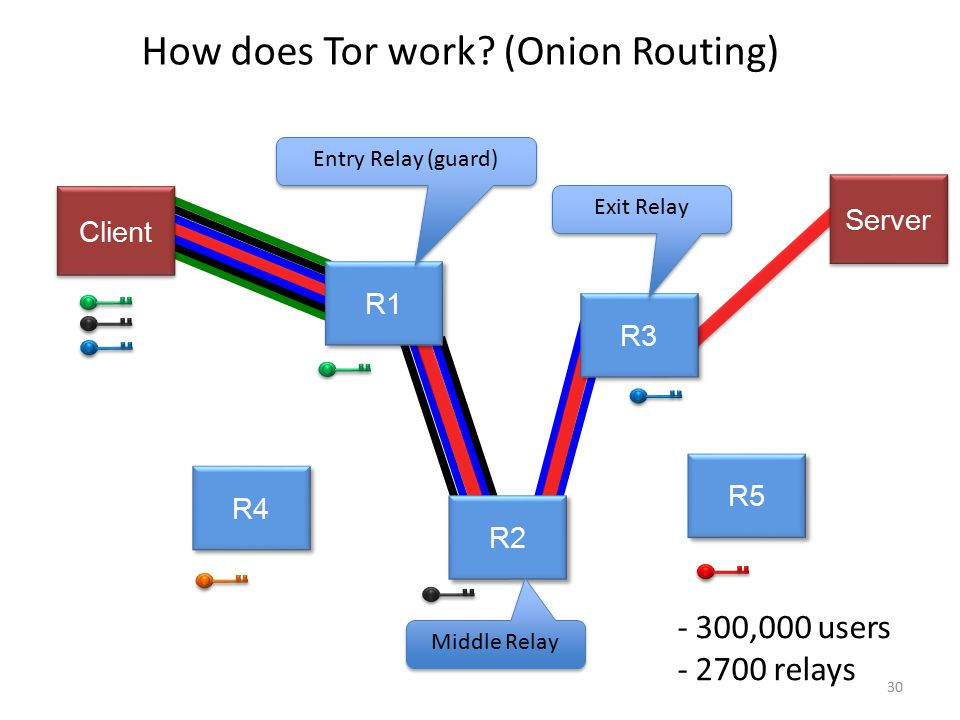
\includegraphics[width=1\textwidth]{tor-prejate}
    \caption{TOR routing schema}
    \label{TOR routing schema}
\end{figure}
 
  \begin{figure}[!htb]
    \centering
    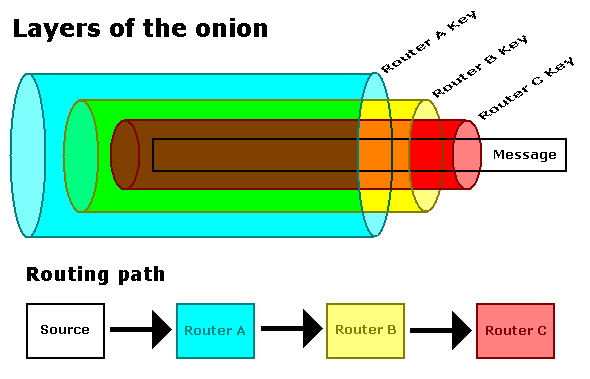
\includegraphics[width=1\textwidth]{tor-packet-prejate}
    \caption{TOR packed encryption schem}
    \label{TOR packed encryption schema}
\end{figure}
 
\section{PGP}

PGP is a program for encrypting data and communication between two parties using public key cryptography.
PGP is used for signing, encrypting and decrypting messages, mostly e-mails.
PGP was developed in 1991 as open source, with the intention 
to provide an open widely used standart for encrypted communication.
Nowadays, PGP program is not open source any more, but the standart is used by open source GPG software.

PGP uses public key cryptography, unlike symmetric cryptography, pgp uses two different keys for encrypting and decrypting.
The user generate a pair of keys, public key for encrypting mails sent to them and private key, which the user
 keeps for himself and use for decrypting messages encrypted with associated public key. The user also publish his public
 key, so other users can send him necrypted messages.

PGP is used in the context of online drug markets as a means of communication between vendors and customers.
Both vendor and customer has their public keys published on their profile page and use the public key of the other
party to encrypt messages to them. This enables vendors and sellers to keep their communication private also 
from the administrators of marketplace.

\section{Online cryptomarkets}
A cryptomarket is an online commercial shopping website, usually accesible only via TOR service.
On cryptomarkets, users can sell and buy  drugs, weapons, hacking tools, stolen credit cards,
counterfeit currency, forged documents and other illegal goods and services.
Most cryptomarkets forbid selling the most unambigously harmful goods, such as
 child pornography or hitman services.

\subsection{Escrow}
Escrow service is a service offered by cryptomarket for their customers.
Escrow means, that the money transfered between two actors(vendor and seller) are held by third party(cryptomarket)
 and are released when both of the parties agree, that they are satisfied with the trade.
 Disputes are resolved by the operator of the cryptomarket.

 Using the Escrow service is usually required.
 Some cryptomarkets allow vendors with long history of satisfied customers to bypass escrow service and recieve money immidiately.
 
\subsection{Tumbler}

Bitcoin transactions are publicly available, but it is not easy to identify their owners.
It might seem, that bitcoin transactions are anonymoous, but when user send bitcoins to
someone(exchange) who knows their identity, the reciever can pair the bitcoin address the bitcoins came from
to identity of sender. Although bitcoin users usually use multiple bitcoin addresses, their transactions and addresses are still 
suspectible to blockchain cashflow analysis, which might identify other addresses of the owner of addres we already know.

Bitcoin Tumblers exist in order to prevent such analysis. User sends bitcoins to the tumbler service, the service mix his bitcoins
with bitcoins of other users by performing multiple transactions between it's bitcoin addresses.
The structure of these transactions differs for different tumbler services.
User generate new bitcoin address with no tie to his previous addresses and bitcoins are recieved from the service to this address.
 There also exists peer-to-peer tumblers(CoinJoin,SharedCoin,coinswap),
that enable multiple users to directly create transactions to mix bitcoins among themselves.
The transaction can be performed multiple types with different actors.

\subsection{Vendor's feedback}

Cryptomarkets usually employs reputation systems, where buyers can publish their satisfaction with the vendor.
These systems are similar to systems used in popular e-commerce websites like amazon or e-bay.
Users can give feedback only to vendors with whom thay have traded with.
On some cryptomarkets it is only possible to upvote and downvote vendors, on some others people can
rate different parts of their interaction with seller, like the easyness of communication,
speed of sending the goods and unsuspiciousness of packaging.

\subsection{Valhalla cryptomarket}


\chapter{Methods and tools to get and analyze data}
\section{Obtaining,storing and analyzing blockchain data}
In order to create a tool, that will find data related to bitcoin adresses, we need to store the blockchain locally in that way, that common graph algorithms can be applied.
We ran the official bitcoin daemon (further referenced as bitcoind), to obtain a copy of bitcoin blockchain. Bitcoind store blockchain in multiple *.blk files.
These files have structure, which is unfit for searching, processing and analysis of blockchain, so I used rusty-parser to parse these files and create csv files of transactions, outputs and adresses.

Than we imported these files into neo4j graph database, to have whole transaction graph in one place and be able to compute statistics and heuristics.
All entities in the \ref{neo4jschema} are represented as graph nodes, the relationships between them are edges.
\begin{figure}[!htb]
    \centering
    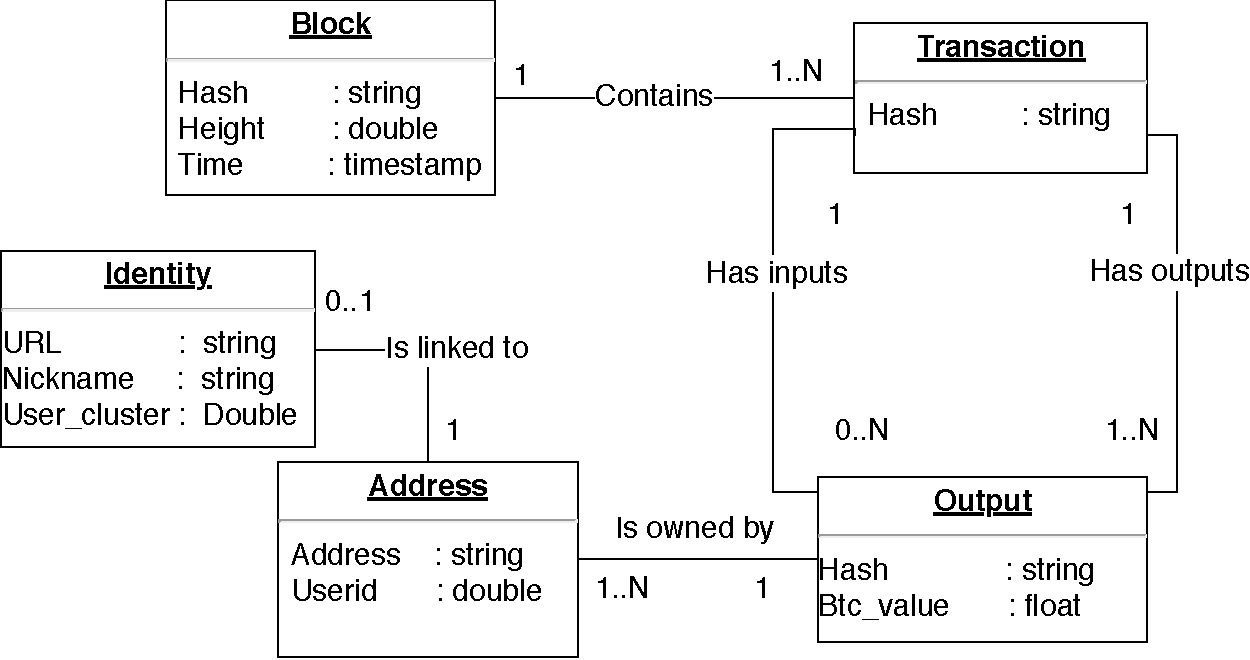
\includegraphics[width=1\textwidth]{neo4j-schema}
    \caption{Neo4j database ER diagram}
    \label{neo4jschema}
\end{figure}

\section{Drug markets web scraping and data collection}
We scraped data from dream market and valhalla, 2 big popular drug markets available via TOR. Wescraped the vendor nicknames, buyer reviews and the sortiment that each vendor sells.
We tested, if every transaction that is happening on drug market has its counter transaction in bitcoin blockchain. Wesent 0.05 bitcoins to both markets,
bought a virtually deliverable legally service(link to secret forum) and checked, if the bitcoins that I have sent to deposit adress left.
For both markets, there was no transaction happening for days after the transaction was done. This means, that markets don't transfer bitcoins,
when there is filled order, all the transactions that these drug markets do are just for depositing bitcoins on drug market account,
withdraw bitcoins and money laundering bitcoins.
We made multiple deposits and withdraws from drug markets in order to track, where were the deposited bitcoins transfered and where the withdrawn bitcoins originated.
These deposits and withdrawals are used to test the resulting application
We scraped 158 vendor PGP keys from dream market and 70 PGP keys from walhalla. Wetested these keys, if they are vulnerable to ROCA attack, via python module roca-detect. None of these keys were vulnerable.
All these PGP keys were searched for User-Id in metadata of PGP key and these user-Ids were seached by google. None of thesearches for user-Ids(both nicknames and mail addresses) returned any results.

We thought that metadata from the photos of drugs, which are available on the drug markets might be useful.
We downloaded hundreds of pictures both from walhalla and dream market.
Only metadata directly dependending on image content(like amount of red, green and blue colors) differ,
metadata that could potentionally help dislosing user identity(date of creation nad modification, signature, software version) were the same.
The software version contained line: $ImageMagick 6.8.9-9 Q16 x86_64 2017-07-31 http://www.imagemagick.org$
We created vendor account on both markets and uploaded an image with custom made metadata to see,
if the metadata were scraped and same version of software version appears. It happened so for both markets,
therefore we believe, that markets automatically scrape metadata from uploaded images in order to protect privacy of the users.

\section{Drug market server fingerprinting}
We tried to scan ports of drug markets servers and fingerprint their webserver, in order to find any vectors of further information gathering.
We scanned both drug markets servers using netcat, finding, that the only opened port is number 443(HTTPS), which is used by webserver.
We used httprecon to fingerprint used HTTP server. The fingerprinting consists of sending multiple malformed HTTP requests and comparing the webserver output with the database of responses by different webservers.
The results of fingerprinting can be see in figure xxx, the best matches are various modern versions of apache webserver.
The results of port scan and webserver printing doesn't indicate any way how to gather data about drug markets servers.

\section{Publicly available data scraping}
In order to have some bitcoind addresses and bitcoins linked to identities, We searched internet for pages, where are bitcoin adresses tied to real or virtual identities.
The interesting sites that I decided to scrape were bitcointalk forum, bitcoin-OTC, reddit, twitter, bitcoin.info.
The bitcointalk and bitcoin-OTC are the most popular internet forums related to cryptocurrencies. The script bitcointalk-scraper.py visits profile pages of all profiles on both forums (even those without any posts)
 and matched with bitcoin address regular expression.
 
The reddit and twitter were scraped by twitter-reddit-scraper.py. The script contain several hardcoded phrases like "Donate bitcoin" and "bitcoind address" and scrapes the results of search page.
Bitcoin.info is a webpage that serves primarly as bitcoin blockchain explorer, secundary,
it gathers multiple statistics about bitcoin blockchain and also offers for third parties to have their bitcoin address and identity listed on their webpage.
Some of these identities are verifies by signaturing custom made message with the bitcoin address associated private key.

We scraped data with the intention to link identities to bitcoin addresses. The data scraped from public sources are rows with thre collums: bitcoin addres, URL where was the addres scraped and username of the associated identity.
All data scraped from the public sources(bitcointalk, reddit,twitter, bitcoin-OTC) are imported to the same neo4j graph database as metadata belonging to the nodes representing given address.


\chapter{Deanonymization techniques}
\section{Detecting wallets owned by drug markets}
\section{Using own transactions to get market wallets}

\chapter{Statistics of drug markets}
Since we are trying to identify 


\section{Methodology}
The data was collected from walhalla drug market on 20.1.2018.
This url's of all market listings are in pattern http://valhallaxmn3fydu.onion/products/xxx where 
xxx is incrementing with each new listing.
We wrote a small script in bash to iterate through all the listings and download them using wget.
To be able to download via wget from .onion links, I had to use privoxy, to redirect the wget through locally ran TOR daemon.
After downloading all the pages of products, we parsed the downloaded files using python and common linux command 
line tools(cat,grep,cut,sed)
From the listing, we parsed vendor's nickname, the subcategory where the listing was placed and title of listing.

By this, we got 666 unique vendors name, so we downloaded and scraped the vendor's profiles pages from the walhalla 
market in similar way.
From the vendor's profile pages, we scraped name of vendor, his total revenue, number of positive and negative reviews 
and the countries from which the vendor ships.
The shortcoming of this method is, that we can download and analyze only sellers, 
that have at least one active listing at the time of data collection. 
Hovewer, we managed to download 20000 listings out of 100000.

The statistics, tables and plots in this chapter were produced by statistical and data analysis software R.
The exact commands to generate these figures and plots can be found in attachments in file named 'valhalla-r.txt'.

\section{Overall statistics of Walhalla drug market}

Walhalla was originally founded as local Finnish market,
that seems the reason for surprisingly many vendors shipping from Finland.
The reader can see the frequency of countries the vendors are shipping from in table \ref{shipcount}.

\begin{table}
    \caption{Countries vendors are shipping from}
    \label{shipcount}
    \begin{tabular}{|l|l|}
    Countries vendors are shipping from\\
      Belgium,Bulgaria,Hungary,Ireland, & 1\\
      Philippines,Romania,Russia,Serbia,Switzerland& 1   \\
        Austria, Czech Republic, India,Spain,Sweden, Argentina  & 2   \\
        Australia                                    & 3   \\ 
        Poland                                       & 4   \\ 
        Canada                                       & 5   \\ 
        France                                       & 6   \\ 
        Norway                                       & 7   \\ 
        Netherlands                                  & 10  \\ 
        Germany                                      & 13  \\ 
        United States                                & 17  \\ 
        United Kingdom                               & 24  \\ 
        Finland                                      & 34  \\ 
        Unknown                                      & 511  
    \end{tabular}
\end{table}

Each circle in \ref{posneg} represents one neighbour and axis represent
the amount of positive and negative reviews that vendor recieved. 
We can see, that vast majority only 2 vendors out of 666 have recieved more negative feedback than positive.
Only 19 vendors out of 666 managed to get more than 50 negative feedbacks, while all of the these 19 vendors had more
 than 400 positive reviews.
Only 40 vendors got more negative feedbacks than positive feedbacks.
 If we look at statistics of reviews from popular e-shop amazon(http://minimaxir.com/2017/01/amazon-spark)
  and consider one and two star reviews as negative, we can see, that amazon sellers on
  average gets between 5-25\% negative reviews, depending on category of the goods.
  On the walhalla market, vast majoririty of sellers have >95\% of positive reviews, as is shown on \ref{pospercent}.
  Also, only 40 vendors have less than 80\% positive reviews and out of that 36 have less 50 reviews in total.
  These numbers indicate, that the customers of valhalla market are much more picky about the vendor they choose
  than regular e-shop cuystomers. If \ref{Vendors by total revenue}
  

\begin{figure}[!htb]
    \centering
    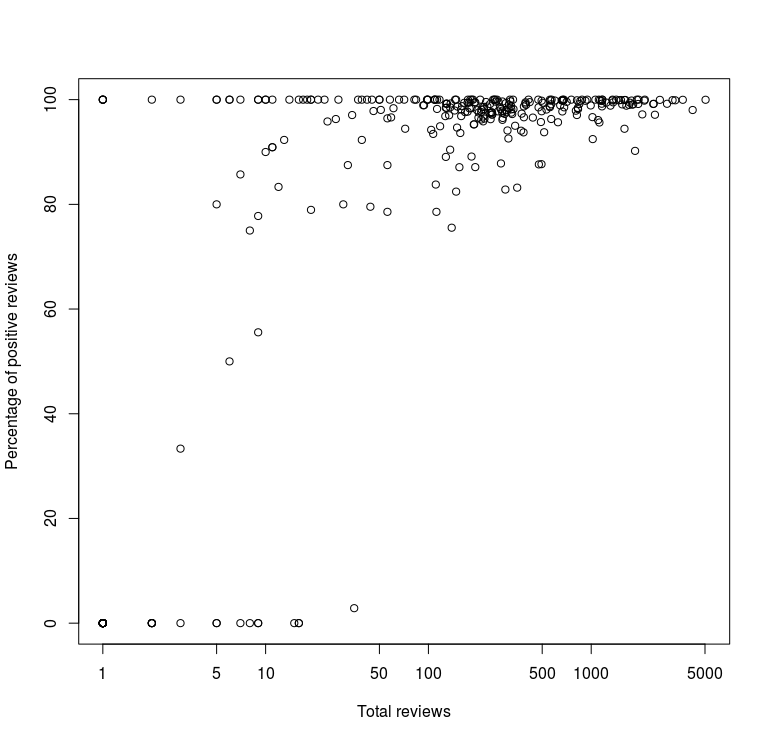
\includegraphics[scale=0.4]{pospercent}
    \caption{Positive reviews of vendors}
    \label{pospercent}
\end{figure}

\begin{figure}[!htb]
    \centering
    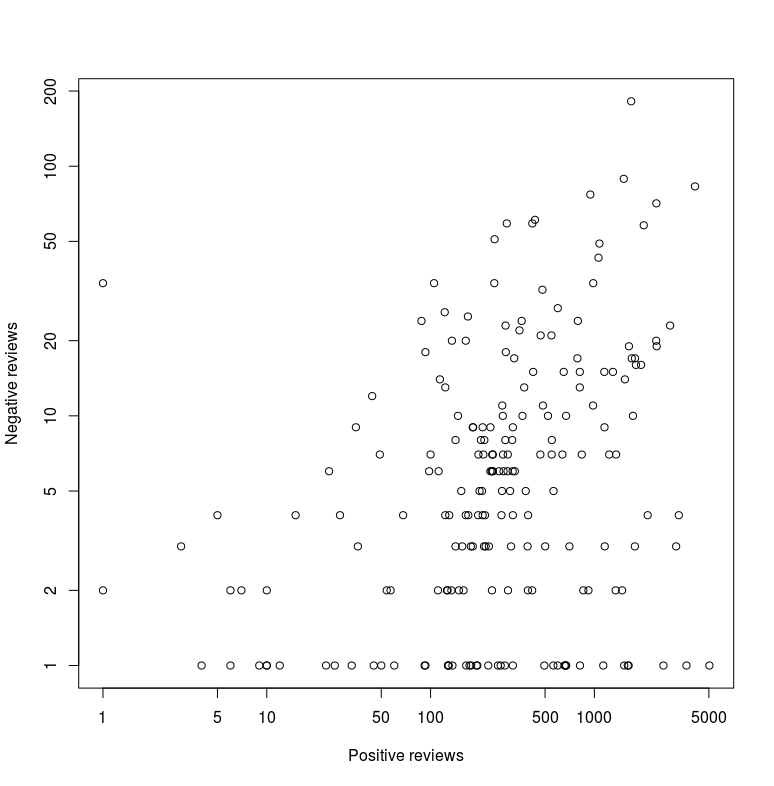
\includegraphics[scale=0.4]{posneg-log}
    \caption{Positive/negative reviews of vendors}
    \label{posneg}
\end{figure}
asfd
\begin{figure}[!htb]
    \centering
    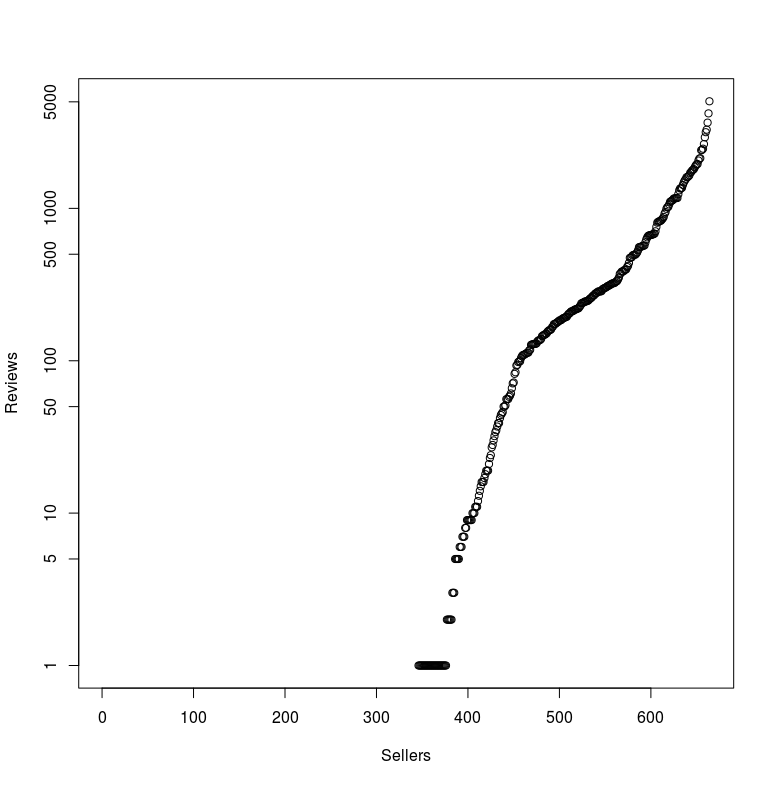
\includegraphics[scale=0.4]{reviews-count-log}
    \caption{Number of reviews for vendors}
    \label{reviews}
\end{figure}
asdf
\begin{figure}[!htb]
    \centering
    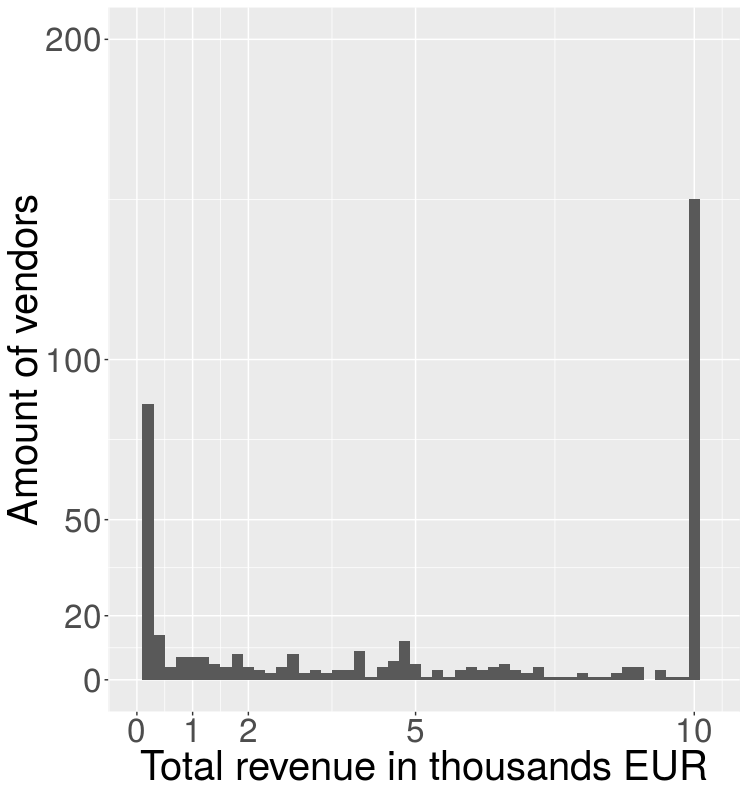
\includegraphics[scale=0.4]{total-rev}
    \caption{Total revenue of vendors}
    \label{Vendors by total revenue}
\end{figure}

\section{Statistics about vendors, drugs availability and distribution and buyers satisfaction}



\chapter{Application}

This chapter describes the application for investigating bitcoin address.
The application consists of three parts.
The scraping module, that downloads bitcoin blockchain and also scrape data from publicly available sites mention in section XXX.
The computanional module, which imports data to the database and also transform data. so that searching in these data would be fast.
The scraping, import and computanional modules are available for linux only.
The GUI written in HTML/JS/CSS, that is connecting to neo4j database REST endpoint and provides visualisation of data.
The GUI can be given a configuration string, to connect to neo4j REST API endpoint, so the gui can be viewed in broser from any device, as long as 
the server with neo4j data is reachable from that device.


\section{Implementation}

The importing module is responsible for parsing bitcoin blockchain files and importing the data into neo4j database.
The importing module take two parameters, the directory of .blk files, which store blockchain data and directory for creating neo4j graph database.
The import module firstly parses the .blk files and save blockchain as multiple .csv files. This intermidiary step is useful for debugging and also simplifies importing to neo4j database.

\begin{figure}[!htb]
    \centering
    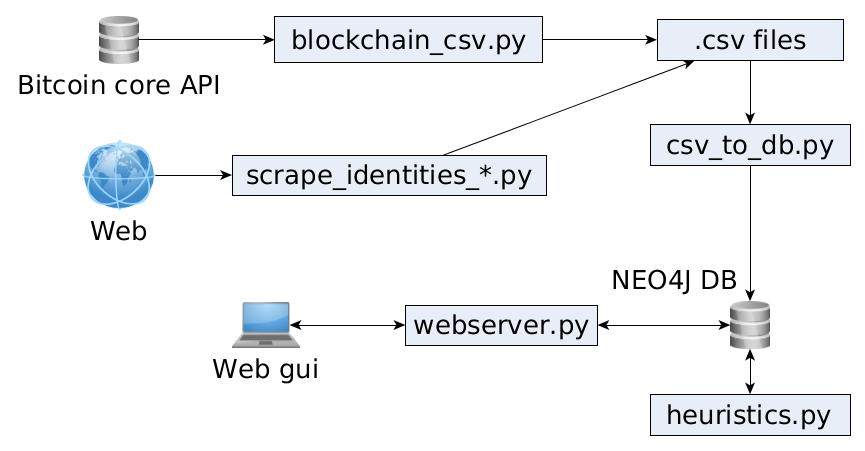
\includegraphics[width=1\textwidth]{application_architecture}
    \caption{Neo4j database ER diagram}
    \label{application_architecture}
\end{figure}

The next importing script is scrape\_identities.py script, which crawl popular forums and multiple websites and creates identities.csv.
File identities.csv contains 3 collumns.
\begin{itemize}
  \item Address - bitcoin address the identity is associated with
  \item Identity - String representing identity, usually username
  \item URL - Url where the Identity and Address were scraped
\end{itemize}

If the user has his own data about the owners of different bitcoin addresses, he can import it through the web GUI later.


\section{Usage}

\noindent See the following command :
\begin{lstlisting}[language=bash]
  $ ./import_module ~/.blockchain/ ~/neo4j/graph.db
\end{lstlisting}

\section{Future development possibilities}


\chapter{Testing and verification of the created tool}
This chapter describes the way, the POC application was tested.

The testing were performed by sending bitcoins to drug markets and withdrawing them.
Than marking the addresses from where the bitcoins were recieved as 

\section{Method of testing}
\section{results}



\chapter{Conclusion}

Here you can insert the appendices of your thesis.gg

\printbibliography
\end{document}
